\documentclass{article}
\usepackage[utf8]{inputenc}
\usepackage[a4paper,left=2.5cm,right=2.5cm,top=2.5cm,bottom=2.5cm]{geometry} 

\usepackage{natbib} % we need this so we can use citation and bib properly
\usepackage{enumitem} % allow you to customize your items (like margins etc.)
\usepackage{xurl} % allow URL breaks at any alphanumerical character
\usepackage{hyperref} % allows you to add hyperlink
\usepackage{amsmath} % allows you to use most mathematical features
\usepackage{float,fancyhdr}
\usepackage{amssymb}
\usepackage{setspace} % allows you to change the line spacing
\usepackage{xcolor}
\usepackage{graphicx} % we need this so we can add figures
\usepackage{booktabs}

\title{Conflict Driven Evolution and Urban Development: \\ Evidence from the Holy Roman Empire\footnote{
I thank Davide Cantoni, Matthias Weigand, and my RA colleagues at the Chair of Economic History for helpful comments and feedback. I thank Matthias Weigand in particular for providing me with his own data and for pointing me towards the paper by \cite{schoenholzer2022}.
}
}
\author{Elias Hadj Ammar}
\date{May 2023}

\begin{document}
\onehalfspacing
\maketitle
\thispagestyle{empty}

\begin{abstract}
How does switching between states affect the long-run development of cities, and why? I study this question in the setting of the Holy Roman Empire, using historical data on construction activity and the territorial history of cities. I specifically test the hypothesis that competition between states, in which higher-quality states dominated, caused cities to benefit from permanent ownership changes. I find evidence in support of this.
\end{abstract}

\newpage

\setcounter{page}{1}
\doublespacing


% ######################################################

\section{Introduction}



The European state system was forged in conflict. No other continent at any time experienced more war than Europe in the early modern era (\citealp{voigtlnder2013}, p. 174). Wars brought death and devastation to the societies affected by them, but their effects also manifested on the political map --- they play out in a diverse ecosystem of polities that come and go and change size over time. Borders get redrawn and territory changes hands. One can indeed imagine this as an evolutionary process: states compete for resources and powerful states eventually absorb weaker ones. As a result, traits that increase state power --- the ability to win conflicts against rivals --- get selected for, while unfavourable traits are doomed to disappear \citep{levine2021}.

In this paper I study the role of this process in the economic development of Europe. In particular, I estimate the effect of state power, the trait that conflict selects for, on urban development. If the effect is positive, then the conflict driven evolution of states may partially explain the eventual ascendancy of Europe: by selecting for military success, Europe's violent history may have accidentally produced fiscal capacity, efficient legal systems, and prospering middle classes.

I build my paper on the theory of conflict driven evolution, outlined above, developed by \cite{levine2013, levine2021, levine2022}. Its main contribution is to explain why hegemonies arose in East Asia while balances of power could prevail in Europe: unlike China, the major powers of continental Europe were frequently preyed upon by strong outsiders --- the Vikings, the Swedes, and the English --- which prevented any one state from growing too strong (\citealp{levine2021}, p. 439). It is worth highlighting how the authors model war between states: you win with state power, and state power is simply free resources, i.e. resources above subsistence. If the most successful states are the ones with the biggest surplus, selection should have made Europe increasingly prosperous.\footnote{The basic idea of Darwinian selection has previously been borrowed by economists - for example \cite{galor2002} do the literal version, where humans are subject to selection and accumulate favourable traits over the course of history. More infamously, \cite{clark2007} employs it in an attempt to explain why the Industrial Revolution took place in Europe, arguing that the rich out-bred the poor and passed favourable traits on to their offspring (in Europe but not elsewhere for some reason.)}

The idea that war and conflict can raise the standard of living dates back to \cite{malthus1798}. He reasoned that "positive checks" on the population (war, disease, famine) lead to higher land-labour ratios and therefore higher levels of income per capita. \cite{voigtlnder2013} build upon this Malthusian mechanism and add an explanation for the incessant wars: taxes on those higher incomes filled the treasuries of the rulers, which increased their demand for war --- a luxury good ---, which in turn kept population low. 

My story is not about population but institutions (although it is compatible with Malthusianism). A longstanding tradition in economics emphasises the role of institutional factors in long-run growth (e.g. \cite{north1970}, \cite{delong1993}, \cite{ajr2001}). From this vast literature one theme is especially relevant here: the institution of fiscal capacity, or the state's ability to collect taxes. \cite{tilly1985} argues that the main reason for states to collect taxes is to be able to wage war. In other words, fiscal capacity and state power are tightly linked --- so if conflict selects for state power, then it also selects for fiscal capacity. \cite{gennaioli2015} and \cite{cantoni2023} show that conflict drove state consolidation. \cite{dincecco2012} show that fiscal capacity had a positive effect on growth.

\cite{diamond1997} and \cite{landes1969, landes2006} have argued for the economic benefits of political fragmentation and state competition. \cite{diamond1997} asserts that geography 
remoteness of China deprived it of the benefits of state competition that European states enjoyed throughout their history. \cite{landes2006} makes a similar argument, pointing out how the totalitarianism and bureaucratism that stifled the spread of innovation in medieval China would not have survived long in a more fragmented state system. Fragmentation also plays a central role in \cite{cervellati2022}'s theory.

The closest relative to this paper is \cite{schoenholzer2022} who investigate how switching between states affects the development of cities. They find that switching states affects population negatively in the short run but positively in the long run. Similar to the evolution metaphor, they interpret this as "creative destruction": the short run cost of destruction is compensated by the long-run benefit of becoming part of a higher-quality state. However, they do not show explicitly how these improvements in state quality are driven by selection through conflict. They use a dataset with a bigger geographical scope (all of Europe) but lower resolution: they use urban population from \cite{bairoch1988} as a proxy for development, which is only available in intervals of 50 or 100 years, and a series of political maps. 

The analysis in this paper builds upon that of \cite{schoenholzer2022} and extends it by identifying special cases of switching events: in \textit{conquests} a city is forcefully absorbed into a new state, while in \textit{successions} a city is absorbed into a new state after the rulers of the old state have gone extinct. Comparing the effects of these two types of switches allows me to tease out the effect of state power. Identification is based on the assumption that conquests imply state power differentials but successions do not. Specifically, if we consider the universe of all switching events, the average increase in state power from the old to the new owner would be higher for the conquests than for the successions. The reasoning is that conflict --- as in a conquest --- selects the new state for power, but conflict-free successions, depending mainly on dynastic marriages, are more "random". This assumption allows me to use conquests as a stand-in for an increase in state power. Several other assumptions are needed to interpret my results causally.

While I am able to replicate \cite{schoenholzer2022}'s result that the long-run effect of switching to another state is positive, I fail to identify a statistically significant effect of state power on urban development. This does not necessarily mean that conflict-driven evolution played no role in the rise of Europe --- several issues limit the statistical power of my test, which might prevent me from finding an effect even if there is one. The biggest one is that the data I use is arguably inadequate for answering the research question.

The rest of the paper proceeds as follows. Section 2 presents some background information. Section 3 describes the data used in the analysis. Section 4 details the empirical approach. Section 5 presents results. Section 6 discusses implications and robustness of the results. Section 7 concludes.

% ######################################################

\section{Background}


One paragraph about the history of Europe's state system; this is the place for Cervellati

One story about a city's territory switch

Two pithy figures, and a no-nonsense table

NO MORE THAN TWO PAGES TOTAL

% ######################################################

\section{Data}

I use data from the \textit{Princes and Townspeople} database which is largely based on the \textit{Deutsches Städtebuch} \citep{keyser1939} and \cite{kobler2007}'s \textit{Historisches Lexikon der Deutschen Länder}. The specific datasets I use are those on city locations \citep{pt1}, territorial histories \citep{pt2}, construction activity \citep{pt5} and conflict incidents \citep{pt6}.\footnote{I thank Davide Cantoni and Matthias Weigand for giving me access to unpublished yearly versions of the construction and territorial histories data.} I aggregate data from these sources to obtain a city-by-year panel of switching events, construction activity, and conflict. 

Switching: describe format; total number of recorded switches; territory id.

Construction: describe format / split and rationale. This can be two paragraphs.

Conflict: describe format (just a dummy).


I also build coarsened versions of this dataset in which I aggregate years into longer periods (10, 50, and 100 years). Not only does this aggregation make event studies nicer to look at, it also allows me to use more of the conflict and construction data as periods get longer: the 50-year and 100-year versions contain events that aren't recorded with a precise year, but only "beginning of the 16th century" and the like. While the 1-year and 10-year data builds contain BLANK construction events with sufficiently precise timing, the 50-year version contains BLANK and the 100-year version contains BLANK.


% ######################################################

\section{Empirical strategy}

\subsection{Long-run effect of switching}

First I replicate the long-term finding of \cite{schoenholzer2022} using the following equation:

\begin{equation}
    construction_{it} = \alpha_i + \delta_t + \mathbf{1}(S_{it} > 0) + 
    \sum_{\tau = -100}^{200} \mathbf{1}(t = e^{NewState}_i + \tau)\pi_t + \varepsilon_{it}
\end{equation}


\subsection{Effect of state power}


Next I tried to find the effect of state power - the effect of the difference in selection for state power between conquests and successions:

I use a triple interaction. I extend the previous regression

\begin{multline}
    construction_{it} = \alpha_i + \delta_t + \mathbf{1}(S_{it} > 0) +
    \mathbf{1}(t \ge e^{NewState}_i)\beta +
    \mathbf{1}(t \ge e^{NewState}_i) \times C_i \times \theta + \varepsilon_{it}
\end{multline}



Blah blah.


\section{Results}

I can barely believe it myself, but I replicate their finding. Table 
Figure \ref{fig:SW_replication} shows the dynamic effect of switching. Cities were on average 

The it's not as convincing: \ref{tab:SW22_replication_50y}



\newpage
\onehalfspacing
\bibliographystyle{chicago}
\bibliography{references.bib}

\newpage
\section*{Tables and figures}

\subsection*{Tables}

\begin{table}[htbp]
   \caption{\label{tab:SW22_replication_50y} Dynamic effects of switching}
   \centering
   \begin{tabular}{lcccc}
      \tabularnewline \midrule \midrule
      Dependent Variables:            & All construction & State  & Private & Public goods\\  
      Model:                          & (1)              & (2)    & (3)     & (4)\\  
      \midrule
      \emph{Variables}\\
      Treat $\times$ Period $=$ -100  & 0.00             & 0.02   & -0.01   & 0.00\\   
                                      & (0.03)           & (0.02) & (0.01)  & (0.02)\\   
      Treat $\times$ Period $=$ 0     & 0.00             & 0.02   & 0.00    & -0.02\\   
                                      & (0.02)           & (0.02) & (0.01)  & (0.01)\\   
      Treat $\times$ Period $=$ 50    & 0.02             & -0.01  & 0.01    & -0.03$^{**}$\\   
                                      & (0.02)           & (0.02) & (0.01)  & (0.01)\\   
      Treat $\times$ Period $=$ 100   & 0.05$^{**}$      & 0.01   & 0.00    & 0.00\\   
                                      & (0.03)           & (0.02) & (0.01)  & (0.02)\\   
      Treat $\times$ Period $=$ 150   & 0.05$^{*}$       & -0.01  & 0.02    & 0.00\\   
                                      & (0.03)           & (0.02) & (0.02)  & (0.02)\\   
      Treat $\times$ Period $=$ 200   & 0.09$^{***}$     & 0.03   & -0.01   & -0.01\\   
                                      & (0.03)           & (0.03) & (0.02)  & (0.02)\\   
      Switching indicator             & -0.01            & 0.01   & -0.01   & 0.00\\   
                                      & (0.02)           & (0.02) & (0.01)  & (0.01)\\   
      \midrule
      \emph{Fixed-effects}\\
      City                            & Yes              & Yes    & Yes     & Yes\\  
      Period                          & Yes              & Yes    & Yes     & Yes\\  
      \midrule
      \emph{Fit statistics}\\
      Observations                    & 6,635            & 6,635  & 6,635   & 6,635\\  
      R$^2$                           & 0.3563           & 0.2799 & 0.3260  & 0.2916\\  
      Within R$^2$                    & 0.0024           & 0.0013 & 0.0007  & 0.0010\\  
      \midrule \midrule
      
      
   \end{tabular}
   
   \par \raggedright 
   Note: Table presents results of estimation equation \eqref{eq:sw22}. Yearly data was aggregated into periods of 50 years. Observations are at the city-period  level. Dependent variables are indicators that take the value 1 if  construction activity of the respective type was recorded. Standard errors are  clustered at the city level. *, **, and *** denote significance on the 10 percent, 5 percent, and 1 percent  level, respectively.
\end{table}


\begin{table}[htbp]
   \caption{Test Title}
   \centering
   \begin{tabular}{lcc}
      \tabularnewline \midrule \midrule
      Dependent Variable: & \multicolumn{2}{c}{Construction}\\
      Model:                                               & (1)           & (2)\\  
      \midrule
      \emph{Variables}\\
      Switching to another state $\times$ Selection $=$ 1  & 0.01 (0.03)   & 0.04 (0.05)\\   
      Switching to another state $\times$ Selection $=$ 3  & 0.04 (0.04)   & -0.15$^{***}$ (0.06)\\   
      Switching to another state                           & 0.02 (0.03)   & -0.010 (0.05)\\   
      Switching indicator                                  & -0.008 (0.03) & -0.09 (0.06)\\   
      Conflict                                             &               & 0.01 (0.03)\\   
      \midrule
      \emph{Fixed-effects}\\
      City                                                 & Yes           & Yes\\  
      Period                                               & Yes           & Yes\\  
      \midrule
      \emph{Fit statistics}\\
      Observations                                         & 6,635         & 1,955\\  
      R$^2$                                                & 0.3553        & 0.4245\\  
      Within R$^2$                                         & 0.0009        & 0.0071\\  
      \midrule \midrule
      \multicolumn{3}{l}{\emph{Clustered (City) standard-errors in parentheses}}\\
      \multicolumn{3}{l}{\emph{Signif. Codes: ***: 0.01, **: 0.05, *: 0.1}}\\
   \end{tabular}
\end{table}


\clearpage
\subsection*{Figures}

\begin{figure}
    \centering
    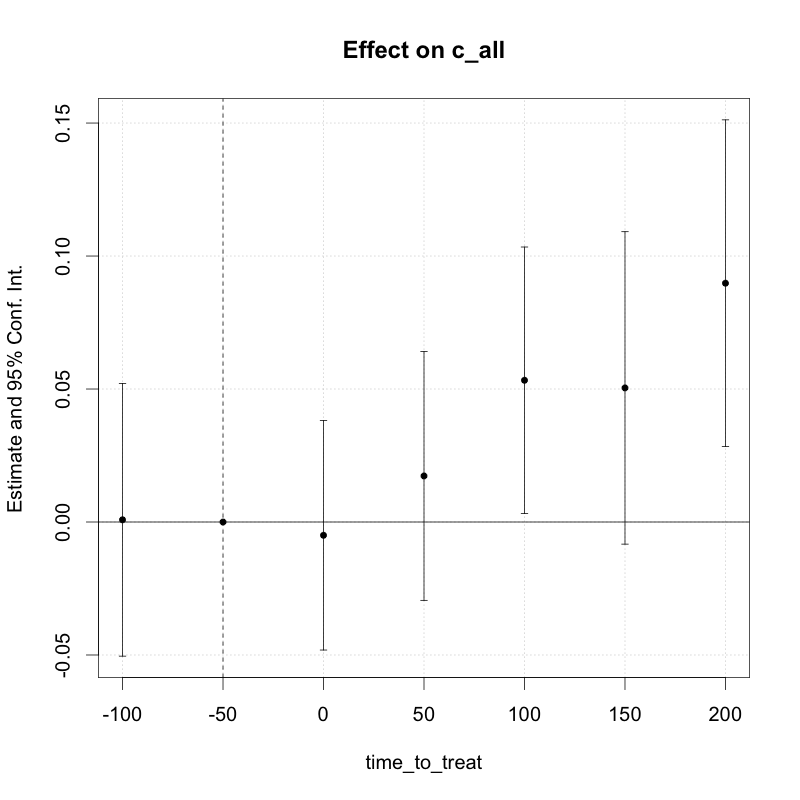
\includegraphics[scale = 0.4]{paper/output/regressions/SW22_replication_50y.png}
    \caption{It looks just like it's supposed to!}
    \label{fig:SW_replication}
\end{figure}




\end{document}
